\documentclass[10pt]{article}

% --- Packages ---
\usepackage[utf8]{inputenc}
\usepackage{amsmath, amssymb, amsthm}
\usepackage{asymptote}
\usepackage{geometry}
\usepackage{fancyhdr}
\usepackage{graphicx}
\usepackage{tikz}
\usepackage{enumitem}
\usepackage{hyperref}
\usepackage{xcolor}
\usepackage{indentfirst}
\usepackage{pgfplots}
\pgfplotsset{compat=1.18}

% --- Page Setup ---
\geometry{margin=1in}
\pagestyle{fancy}
\fancyhf{}
\rhead{Qinghao Hu}
\lhead{AOPS}
\cfoot{\thepage}

% --- Theorem Environments ---
\newtheorem{theorem}{Theorem}[section]
\newtheorem{definition}[theorem]{Definition}
\newtheorem{lemma}[theorem]{Lemma}
\newtheorem{proposition}[theorem]{Proposition}
\newtheorem{corollary}[theorem]{Corollary}
\theoremstyle{remark}
\newtheorem*{remark}{Remark}
\newtheorem*{example}{Example}

% --- Custom Commands ---
\newcommand{\R}{\mathbb{R}}
\newcommand{\N}{\mathbb{N}}
\newcommand{\Z}{\mathbb{Z}}
\newcommand{\Q}{\mathbb{Q}}
\newcommand{\C}{\mathbb{C}}
\newcommand{\ds}{\displaystyle}

% --- Title ---
\title{\textbf{AOPS AMC12 class Note 2} \\ \large functions}
\author{Qinghao Hu}
\date{\today}

\begin{document}

\maketitle
\newpage
\tableofcontents
\newpage

%this is for section one
\section{Class 1: Quadratics, Vieta, and Factorization}
Today, we will look at quadratic functions, Vieta's formula and factorizations

\subsection{Quadratic Equation}

\textit{A quadratic equation is an equation of the form}

\begin{equation}
	ax^2 + bx + c = 0
\end{equation}

\textit{where a, b and c are constants and $a \ne 0$ }
\\\\

\subsection{Roots of Quadratic Equation}

\textit{The roots of Quadratic Equation can be determined by the Quadratic Formula, or more formally, Sridharacharya Formula}
\\
\\
\textit{Assume $r_1$ and $r_2$ are both roots of the Quadratic Equation $ax^2 + bx + c = 0$}

\begin{equation}
	r_1 = {{-(b) + \sqrt{b^2 - 4ac}} \over 2a}, r_2 = {{-(b) - \sqrt{b^2 - 4ac}} \over 2a}
\end{equation}

\textit{$r_1$ and $r_2$ may be imagery numbers if $\sqrt{b^2 - 4 a c} < 0$}
\\\\

\subsection{Vieta's Formula}
\textit{Assume we have a polynomial formula with degree of n}

\begin{equation}
	P(x) = a_n{x^n} + a_{n - 1}{x^{n-1}} + \cdots + a_1x + a_0
\end{equation}

\textit{and $r_1, r_2, \cdots, r_n$ are the roots of the polynomial}
\\
\textit{we can get:}

\begin{equation}
	r_1 + r_2 + \cdots + r_{n - 1} + r_n = {a_{n - 1} \over a_n} \\
\end{equation}

\begin{equation}
	(r_1r_2 + r_1r_3 + \cdots + r_1r_{n-1} + r_1r_n) + (r_2r_3 + r_2r_4 + \cdots + r_2r_{n-1} + r_2r_n) + \cdots + r_{n - 1}r_n  = {a_{n - 2} \over a_n}
\end{equation}

\begin{equation}
	r_1r_2\cdots r_{n-1}r_n = {(-1)^n{a_0 \over a_n}}
\end{equation}
\\\\

\subsection{Factorizations}
\textit{Some key factorizations that you should be familiar with are different of square, difference of cubes, and sum of cubes}
\\\\

one good example is the "Simon's favorite factoring trick"
\\\\
for example:
\\
\begin{center}
Factor the equation, $mn - 2m - 4n + 8 = 8$
\end{center}

we can get:
\begin{center}
	(m - 4)(n - 2) = 8
\end{center}

\newpage

\section{Class 2: Solving equations and systems}
\begin{center}
	\textbf{Summary:}	
	\\
	When dealing with several variables, look for ways of eliminating them to get what you want. And make sure you read the problem carefully so that you know what you want,
	and you do not end up doing more work than you have to. 
\end{center}

\newpage
\section{Class 3: Sequences and Series}

\subsection{Arithemtic Sequences and Series}
An arithmetic sequence is a sequence of the form $a,a+d,a+2d$, and so on (for example, 7,11,15,19 is an arithmetic sequence).
In other words, we begin with a first term a, and repeatedly add a common difference d to obtain the terms that follow.
\\

Te sum of the arithmetic series with n terms is:
\begin{equation}
	a + (a + d) + \cdots + [a + (n - 1)d] = {{2a + (n - 1)d} \over 2} * n
\end{equation}

\subsection{Geometric Sequences and Series}

A geometric sequence is a sequence of the for $a, ar, ar^2$, and so on. 
In other words, we have a first term $a$, and repeatedly multiply by a common ratio $r$ to obtain the terms that follow
\\

\textbf{The sum of the geometric series with n term is: }
\begin{equation}
	a + ar + \cdots + ar^{n - 1} = {{a(r^n - 1)} \over r - 1} = {{a(1 - r^{n})} \over {1 - r}}
\end{equation}

\textbf{The numerator can be viewed as the difference of two terms, $a$ and $ar^n$.}\\
\underline{Notice in particular that these are not the first term and last term.}
\newline

For $|r| < 1$, the sum of the infinite geometric series is:
$$a + ar + ar^2 + \cdots = {a \over {1 - r}}$$ 
\newpage
% Lesson 4
\begin{center}
\section{Lesson 4: Functions and Polynomials}
\end{center}
Today we will look at the properties of certain functions, such as the "floor" function and logarithm, as well as polynomials,
which form a very special class of functions
\newline

\subsection{ABSOLUTE VALUE}
\textit{The absolute value signs make equation difficult to work with. How might we deal with those pesky bars ($|a|$)} \newline

\begin{example}
if $x < 0$, then what happens to the equation $|x| + x + y = 10$, if $x > 0$, then what happens to the equation $[x] + x + y = 10$
\end{example}

\begin{center}
\begin{tikzpicture}[scale=0.8]
  \draw[->] (-3.5,0) -- (3.5,0) node[right] {$x$};
  \draw[->] (0,-0.5) -- (0,4) node[above] {$y$};
  \draw[domain=-3:3, variable=\x, smooth, thick, blue] 
    plot ({\x}, {abs(\x)});
  \node at (2,2) [right] {$y = |x|$};
\end{tikzpicture}
\end{center}

\subsection{Floor Function}
In case you have not seen it before, $\left \lfloor x \right \rfloor$ is the greatest integer less than or equal to x, also called the floor of x. In other words, 
$\left \lfloor x \right \rfloor$ is $x$ rounded down to the nearest integer.
\begin{center}
(In general \\
	$\left \lfloor x + n \right \rfloor\ = \left \lfloor x \right \rfloor + n$ \\	
for any integer $n$)
\end{center}

\subsection{Logarithms}
\textit{Logarithms identity:}
\begin{center}
	$\log_{b}{x} + \log_{b}{y} = \log_{b}{xy}$ \textbf{(Product law)}\\
	$\log_{b}{x} - \log_{b}{y} = \log_{b}{\frac{x}{y}}$ \textbf{(Quotient Law)}\\
	$\log_{b}{x^n} = n\log_{b}{x}$ \textbf{(Power law)}\\
	$\log_b{x} = \frac{\log_a{x}}{\log_a{b}}$ \textbf{(Power Law)}\\
	$\log_{b^n}{x^n} = \log_{b}{x}$\\
\end{center}

\subsection{POLYNOMIALS}
Let $F(x)$ and $G(x)$ be polynomials. If we divide $G(x)$ into $F(x)$, then we will obtain a quotient $Q(x)$
and a remainder $R(x)$, where the degree of $R(x)$ is less than the degree of $G(x)$. The quotient $Q(x)$ and 
$R(x)$ are unique. \\

Also, if a polynomial has all real coefficients, then its nonreal roots must come in conjugate pairs. (\textit{Complex Conjugate Root Theorem})
\\
\\
if:
\[
	c_nx_n^{e_n} + c_{n - 1}x_{n - 1}^{e_{n - 1}} + \cdots + c_0x_0^{e_0} = 0
\]
and
\begin{center}
	for i from \{0 to $n$\}:
\end{center}
\[
	i \in \R
\]
We can get:
\begin{center}
	if $a + bi$ is a root for the polynomial, $a - bi$ will also be the root of the polynomial
\end{center}

%section 5:Tools of Algebra
\newpage
\section{Tools for Algebra}
Today, we will look at what we will describe as the tools of algebra. This tools include working with radicals (square roots and cube roots), and finding the extrema (minima 
maxima) of functions\\

\subsection{RADICALS}
\begin{example}
	1. What does $\frac{2\sqrt{6}}{\sqrt{2} + \sqrt{3} + \sqrt{5}}$ equal to\\
	\textit{To solve this problem, we need to rationalize this term.}
	\textit{Why not we multiple both numerator and denominator by $(\sqrt{2} + \sqrt{3} + \sqrt{5})$}
	\[
		\frac{2\sqrt{6}}{\sqrt{2} + \sqrt{3} + \sqrt{5}} = \frac{2\sqrt{6} * (\sqrt{2} + \sqrt{3} - \sqrt{5})}{(\sqrt{2} + \sqrt{3} + \sqrt{5})
		* (\sqrt{2} + \sqrt{3} - \sqrt{5})}
	\]
	\textit{We can expand the denominator using difference of squares:}\\
	\[
		(\sqrt{2} + \sqrt{3} + \sqrt{5}) * (\sqrt{2} + \sqrt{3} - \sqrt{5}) = (\sqrt{2} + \sqrt{3}) ^ 2 - (\sqrt{5})^2
	\]
	\textit{We expand, we will get:}
	\[
		(\sqrt{2} + \sqrt{3}) ^ 2 - (\sqrt{5})^2 = 2 + 2\sqrt{6} + 3 - 5 = 2\sqrt{6}
	\]
	\textit{Finally:}
	\[
		\frac{2\sqrt{6} * (\sqrt{2} + \sqrt{3} - \sqrt{5})}{2\sqrt{6}} = (\sqrt{2} + \sqrt{3} - \sqrt{5})
	\]\\
\end{example}

\begin{example}
	2. Which of the following is closest to $\sqrt{65} - \sqrt{63}$?\\
	We can use a less common technique that is called "Rationalize the numerator"
	\[
		\frac{\sqrt{65} - \sqrt{63}}{1}
	\]
	Rationalize the numerator, we get:
	\[
		\frac{(\sqrt{65} - \sqrt{63}) * (\sqrt{65} + \sqrt{63})}{(\sqrt{65} + \sqrt{63})} = \frac{2}{\sqrt{65} + \sqrt{63}}
	\]
	$\sqrt{65} + \sqrt{63}$ is quite close to 8 + 8. So our fraction is really close to $\frac{2}{8 + 8} = 0.125$. It's really close to the (A) and (B) options.\\
	What can we do to find out whether $\sqrt{65} + \sqrt{63}$ is a little more or a little less than 8 + 8\\ 
	We can graph the function $f(x) = \sqrt{x}$:\\
	\begin{center}
	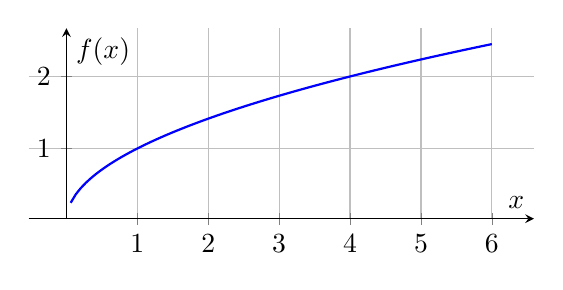
\begin{tikzpicture}
	  \begin{axis}[
	    axis lines = middle,
	    xlabel = $x$,
	    ylabel = {$f(x)$},
	    domain=-1:6,
	    samples=100,
	    grid = both,
	    width=8cm,
	    height=4cm,
	    enlargelimits
	  ]
		  \addplot[blue, thick] {sqrt(x)};
	  \end{axis}
	\end{tikzpicture}
	\end{center}
	The root function $y = \sqrt{x}$ is getting less and less steep as x increases.\\
	So $\sqrt{65} - \sqrt{63}$ is less than 16\\
	$\therefore$ the number should be greater than $0.125$\\
	Choose (B)\\
	\\
\end{example}

\begin{example}
	If 
	\[
		N = \frac{ \sqrt{ \sqrt{5} + 2} + \sqrt{\sqrt{ 5 } - 2} }{ \sqrt{ \sqrt{5} + 1 } } - {\sqrt{ 3 - 2\sqrt{2}}}
	\]
	the $N$ equals\\
	(A) 1  (B) $2\sqrt{2} - 1$  (C) $\frac{\sqrt{5}}{2}$  (D) $\sqrt{\frac{5}{2}}$  (E) none of these\\
	We can try to rationalize the first section:
	\[
		=\frac{ \sqrt{ \sqrt{5} + 2} + \sqrt{\sqrt{ 5 } - 2} }{ \sqrt{ \sqrt{5} + 1 } } * \frac{\sqrt{\sqrt{5} - 1}}{\sqrt{\sqrt{5} - 1}}
	\]
	\[
		=\frac{\sqrt{3 + \sqrt{5}} - \sqrt{7 - 3\sqrt{5}}}{2}
	\]
	We can go a step forward using radicals\\
	set $a, b, \{a, b \in \mathbb{Q}\}$
	\[
		\sqrt{a} + \sqrt{b} = \sqrt{3 + \sqrt{5}}
	\]
	\[
		a + b + 2\sqrt{ab} = 3 + \sqrt{5}
	\]
	We can list a linear equation system: 
	\[
		\left\{\begin{matrix}
		 a + b = 3\\
		 4ab = 5 \\
		\end{matrix}\right.
	\]
	\[
		a = \frac{1}{2}, b = \frac{5}{2}
	\]
	So,
	\[
		\sqrt{3 + \sqrt{5}} = \sqrt{\frac{1}{2}} + \sqrt{\frac{5}{2}}
	\]
	Apply the rule to all the terms, we can get:
	\[
		\cdots \cdots
	\]
	\[
		\sqrt{2} - (\sqrt{2} - 1) = 1
	\]
	So choose (A)\\
\end{example}

\begin{example}
	3. What is the smallest integer larger than $(\sqrt{3} + \sqrt{2})^6$?\\
	\\
	(A) 972 (B)971 (C)970 (D)969 (E)968
	\[
		(\sqrt{3} + \sqrt{2})^6 = (5 + 2\sqrt{6})^3 = 485 + 198\sqrt{6}
	\]
	It's really hard to say which is it greater than 970\\
	But there is an interesting facto, the conjugate of the number, $\sqrt{3} - \sqrt{2} = 485 - 198\sqrt{6}$
	So,
	\[
		(\sqrt{3} + \sqrt{2})^6 + (\sqrt{3} - \sqrt{2})^6  = (485 + 198\sqrt{6}) + (485 - 198\sqrt{6}) = 970
	\]
	$(\sqrt{3} - \sqrt{2})^6$ is a really small number(less than 1), so $()\sqrt{3} - \sqrt{2})^6$ must between 969 and 970\\ 
	Select (C)\\ 
	\\
\end{example}

\subsection{MINIMA AND MAXIMA}
When give you multiple function and solve for Minima and maxima, just graph it.\\
Think about the elements of Minima and Maxima.\\

\subsection{AM-GM inequality} 
The AM-GM inequality states that the arithmetic mean of any set of nonnegative real numbers is greater than or 
equal to the geometric mean of those numbers.\\ \\
In other words, if $x_1, x_2, \cdots, x_n \geq 0$, then:
\[
	\frac{x_1 + x_2 + \cdots + x_n}{n} \geq \sqrt[n]{x_1*x_2*x_3\cdots x_n}
\]
Equality occurs if and only if $x_1 = x_2 = x_3 = \cdots = x_n$. That is, the arithmetic mean is actually
strictly greater than the geometric mean unless all the numbers are the same.\\

\subsection{THE TRIANGLE INEQUALITY}
Assume a, b and c are sides of a triangle
\begin{gather}
	a + b > c \\
	a + c > b \\
	b + c > a
\end{gather}
\newpage
\section{Triangles}
\subsection{Right Triangles}
In many geometry problems, building right triangles is an important step, because right triangles give us a way of 
computing distances via the \textit{Pythagorean theorem}. It is also important to recognize special triangle, 
suc as the 30-60-90 and 45-45-90 right triangles \\
\begin{example}
	In rectangle $ABCD$, angle $C$ is trisected by $\overline{CF}$ and $\overline{CE}$, where $E$ is on $\overline{AB}$
	, $BE = 6$, and $AF = 2$. Which of the following is closest to the area of the rectangle $ABCD$? 
	unitsize(0.3 cm);

\end{example}
\subsection{Similar Triangle}
When you see a question, try to find similar triangles first. They may help you find information about unknown 
variables. \\

\subsection{Law of Sines and Cosines}
\textbf{Law of Sines} \\ 
In triangle $ABC$, let the sides opposite angle $A$, $B$ and $C$ have lengths $a$, $b$ and $c$
respectively. Then
\[
	\frac{a}{\sin{A}} = \frac{b}{\sin{B}} = \frac{c}{\sin{C}}
\]

\subsection{Law of Cosines}
In triangle $ABC$, let the sides opposite angles $A$, $B$ and $C$ have lengths $a$, $b$ and $c$ respectively. Then
\[
	c^2 = a^2 + b^2 - 2ab\cos{C}
\]

\subsection{Heron's Formula}
Assume $a$, $b$ and $c$ are side lengths of a triangle. Assume $s$ are half of the perimeter of the triangle
\[
	area = \sqrt{s*(s - a) * (s - b) * (s - c)}
\]
\newpage

\section{Circle}
\subsection{Example Question}
Always think about using dot lines to spilit the picture to get datas that are calculatable 

\subsection{Example Question 2}
When we have three circles $a$, $b$ and $c$, and they are tangent to lines or other circles and we have the relationship:

\[
	\frac{1}{\sqrt{a}} + \frac{1}{\sqrt{b}} = \frac{1}{\sqrt{c}}
\]

\subsection{Power of a Point}

Circles have very important properties with respect to angles. They also have important properties with respect to lengths, most notably the **Power of a Point**. \newline
This is what the Power of a Point theorem says: Suppose that $P$ is a point not on a circle $\omega$. Suppose that one line through $P$ 
intersects circle $\omega$ at points $A$ and $B$, and that another line through $P$ intersects the circle at points $C$ and $D$. Then the following holds:

\[
PA \cdot PB = PC \cdot PD
\]

This product is called the **power of point $P$** with respect to the circle.

\subsection{The inradius of a quadrilaterial rectangle}
$r$ is radius of the incircle, $K$ and $s$ are the area and semi-perimeter of the quadrilateral
\[
	r = \frac{K}{s}
\]
\newpage

\section{Class 8: Polygons and Three-Dimensional Geometry}
\subsection{Polygons}
For a regular polygon with $m$ sides, each interior angle measure is equal to $\frac{180(m - 2)}{m}$(in degree), 
which we can also write as $180^{\circ} - \frac{360^{\circ}}{m}$

\newpage
\section{Class 9: Number Theory}

\begin{itemize}
	\item \textbf{Number Theory can be boardly described as the study of the properties of integers, such as divisibility}
	\item \textbf{In number theory, we often restrict our attention to positive integers, but sometimes we must also extend our attention to negative integers as well. Remember to look for presence or absence of the world
	"positive" in the problem statement}
\end{itemize}

For the positive integer $x$, its factor from is 
\[
	x = a_{1}^{e_{1}} * a_{2}^{e_{2}} * \cdots * a_{n}^{e_{n}}
\]
The number of dividend is defined by:
\[
	\text{Number of dividend} = (e_{1} + 1) * (e_{2} + 1) * \cdots\cdots * (e_{n} + 1) 
\]


\end{document}

% Referenc
% \section{Introduction}
% Write your introduction or overview of the day's topic here.
%
% \section{Main Concepts}
% \begin{definition}
% A function \( f: A \to B \) is said to be \textbf{injective} if for every \( a_1, a_2 \in A \), \( f(a_1) = f(a_2) \Rightarrow a_1 = a_2 \).
% \end{definition}
%
% \begin{theorem}
% Let \( f: \R \to \R \) be a continuous and strictly increasing function. Then \( f \) is injective.
% \end{theorem}
%
% \begin{proof}
% Assume \( f(a) = f(b) \). Since \( f \) is strictly increasing, if \( a < b \), then \( f(a) < f(b) \), contradiction. So \( a = b \).
% \end{proof}
%
% \section{Examples}
% \begin{example}
% Let \( f(x) = x^2 \). Then \( f \) is not injective on \( \R \), but it is injective on \( [0, \infty) \).
% \end{example}
%
% \section{Diagrams}
% \begin{center}
% \begin{tikzpicture}[scale=1]
% \draw[->] (-2,0) -- (2,0) node[right] {$x$};
% \draw[->] (0,-1) -- (0,4) node[above] {$y$};
% \draw[domain=-1.5:1.5, smooth, variable=\x, blue, thick] 
%     plot ({\x}, {\x*\x});
% \node at (1.2,3.2) {$y = x^2$};
% \end{tikzpicture}
% \end{center}
%
% \section{Summary}
% Summarize what you learned today.
% \begin{tikzpicture}
%   \begin{axis}[
%     axis lines = middle,
%     xlabel = $x$,
%     ylabel = {$f(x)$},
%     domain=-2*pi:2*pi,
%     samples=100,
%     grid = both,
%     width=12cm,
%     height=6cm,
%     enlargelimits
%   ]
%     \addplot[blue, thick] {sin(deg(x))};
%   \end{axis}
% \end{tikzpicture}
